%%%%%%%%%%%%%%%%%%%%%%%%%%%%%%%%%%%%%%%%%%%%%%%%%%%%%%%%%%%%%%%%%%%%%%%%%%%%%%%%%%%%%%%%%%%%%%%%%%%
%%%%%%%%%%%%%%%%%%%%%%%%%%%%%%%%%%%%%%%%%%%%%%%%%%%%%%%%%%%%%%%%%%%%%%%%%%%%%%%%%%%%%%%%%%%%%%%%%%%
%%%%%%%%%%%%%%%%%%%%%%%%%%%%%%%%%%%%%%%%%%%%%%%%%%%%%%%%%%%%%%%%%%%%%%%%%%%%%%%%%%%%%%%%%%%%%%%%%%%
\documentclass[12pt,dvipdfmx]{beamer}
%%%%%%%%%%%%%%%%%%%%%%%%%%%%%%%%%%%%%%%%%%%%%%%%%%%%%%%%%%%%%%%%%%%%%%%%%%%%%%%%%%%%%%%%%%%%%%%%%%%%%%
% pdfの栞・プロパティの字化けを防ぐ
\usepackage{atbegshi}
%\AtBeginShipoutFirst{\special{pdf:tounicode 90ms-RKSJ-UCS2}} %Windows
\AtBeginShipoutFirst{\special{pdf:tounicode EUC-UCS2}} %Linux, Mac
\usepackage{hyperref}
%%%%%%%%%%%%%%%%%%%%%%%%%%%%%%%%%%%%%%%%%%%%%%%%%%%%%%%%%%%%%%%%%%%%%%%%%%%%%%%%%%%%%%%%%%%%%%%%%%%%%%
%%%
%%% テーマの指定、省略時は default になる
%%%

 % フレームの指定、省略可
%%%%%%%%%%%%%%%%%%%%%%%%%%%% THEME
  %\usetheme{AnnArbor}
  %\usetheme{Antibes}
  %\usetheme{Bergen}
  %\usetheme{Berkeley}
  %\usetheme{Berlin}
  \usetheme{Boadilla}
  %\usetheme{boxes}
  %\usetheme{CambridgeUS}
  %\usetheme{Copenhagen}
  %\usetheme{Darmstadt}
  %\usetheme{default}
  %\usetheme{Dresden}
  %\usetheme{Frankfurt}
  %\usetheme{Goettingen}
  %\usetheme{Hannover}
  %\usetheme{Ilmenau}
  %\usetheme{JuanLesPins}
  %\usetheme{Luebeck}
  %\usetheme{Madrid}
  %\usetheme{Malmoe}
  %\usetheme{Marburg}
  %\usetheme{Montpellier}
  %\usetheme{PaloAlto}
  %\usetheme{Pittsburgh}
  %\usetheme{Rochester}
  %\usetheme{Singapore}
  %\usetheme{Szeged}
  %\usetheme{Warsaw}

% 省略可
%%%%%%%%%%%%%%%%%%%%%%%%%%%% COLOR THEME
  %\usecolortheme{albatross}
  %\usecolortheme{beetle}
  %\usecolortheme{crane}
  %\usecolortheme{default}
  %\usecolortheme{dolphin}
  %\usecolortheme{dove}
  %\usecolortheme{fly}
  %\usecolortheme{lily}
  %\usecolortheme{orchid}
  %\usecolortheme{rose}
  %\usecolortheme{seagull}
  %\usecolortheme{seahorse}
  %\usecolortheme{sidebartab}
  %\usecolortheme{structure}
  %\usecolortheme{whale}

% ヘッダ、フッタ、フレーム等を指定、省略可
  %%%%%%%%%%%%%%%%%%%%%%%%%%%% OUTER THEME
  %\useoutertheme{default}
  %\useoutertheme{infolines}
  %\useoutertheme{miniframes}
  %\useoutertheme{shadow}
  %\useoutertheme{sidebar}
  %\useoutertheme{smoothbars}
  %\useoutertheme{smoothtree}
  %\useoutertheme{split}
  %\useoutertheme{tree}

% タイトル、section, itemize/enumerate 環境、
% theorem 環境、図, 参考文献などのスタイルを指定、
% 省略可
  %%%%%%%%%%%%%%%%%%%%%%%%%%%% INNER THEME
  %\useinnertheme{circles}
  %\useinnertheme{default}
  %\useinnertheme{inmargin}
  \useinnertheme{rectangles}
  %\useinnertheme{rounded}


%\usefonttheme{}	% 省略可
%\logo{}		% 省略可

%%%%%%%%%%%%%%%%%%%%%%%%%%%%%%%%%%%%%%%%%%%%%%%%%%%%%%%%%%%%%%%%%%%%%%%%%%%%%%%%%%%%%%%%%%%%%%%%%%%
%%%%%%%%%%%%%%%%%%%%%%%%%%%%%%%%%%%%%%%%%%%%%%%%%%%%%%%%%%%%%%%%%%%%%%%%%%%%%%%%%%%%%%%%%%%%%%%%%%%
%%%%%%%%%%%%%%%%%%%%%%%%%%%%%%%%%%%%%%%%%%%%%%%%%%%%%%%%%%%%%%%%%%%%%%%%%%%%%%%%%%%%%%%%%%%%%%%%%%%
% navi. symbolsは目立たないが,dvipdfmxを使うと機能しないので非表示に
\setbeamertemplate{navigation symbols}{}

% 各種パッケージ
\usepackage{graphicx}
%\usepackage{url,cite}
\usepackage{amsmath}
\usepackage{amsthm} \theoremstyle{definition} %theorem環境が斜体になるので注意
\usepackage{amssymb} % AMS-TeX
\usepackage{setspace}

% \AtBeginSection[] % Do nothing for \section*
% { \begin{frame}<beamer> \frametitle{}
%    \tableofcontents[currentsection,subsectionstyle=hide]
%  \end{frame} } 

%appendixをページカウントしない
\newcommand{\backupbegin}{
   \newcounter{framenumberappendix}
   \setcounter{framenumberappendix}{\value{framenumber}}
}
\newcommand{\backupend}{
   \addtocounter{framenumberappendix}{-\value{framenumber}}
   \addtocounter{framenumber}{\value{framenumberappendix}} 
}

%%%%%%%%%%%%%%%%%%%%%%%%%%%%%%%%%%%%%%%%%%%%%%%%%%%%%%%%%%%%%%%%%%%%%%%%%%%%%%%%%%%%%%%%%%%%%%%%%%%%%%
% 本文・数式フォント
%\usepackage{palatino,mathpazo}
%\usepackage{times,mathptmx}
\usepackage[varg]{txfonts}
%\usepackage[varg]{pxfonts}

% \mathcal(\cal)の扱い
%\DeclareMathAlphabet{\mathcal}{OMS}{cmsy}{m}{n} %computer modern
%\DeclareMathAlphabet{\mathcal}{OMS}{txsy}{m}{n} %txfont
%\usepackage[psamsfonts]{eucal} % euler

% mathptmx時に数式モードのvをtxfontから借りる
% \DeclareSymbolFont{lettersA}{U}{txmia}{m}{it}
% \SetSymbolFont{lettersA}{bold}{U}{txmia}{bx}{it}
% \DeclareFontSubstitution{U}{txmia}{m}{it}
% \DeclareMathSymbol{v}{\mathalpha}{lettersA}{"33} %"


%上線 widebar, Widebar
\usepackage{accents}
\makeatletter
\def\widebar{\accentset{{\cc@style\underline{\mskip11mu}}}}
\makeatother


%%%%%%%%%%%%%%%%%%%%%%%%%%%%%%%%%%%%%%%%%%%%%%%%%%%%%%%%%%%%%%%%%%%%%%%%%%%%%%%%%%%%%%%%%%%%%%%%%%%%%%
% 定理環境
% \newtheorem{theorem}{Theorem}
% \newtheorem{lemma}[theorem]{Lemma}
% \newtheorem{corollary}[theorem]{Corollary}
% \newtheorem{definition}[theorem]{Definition}
% \newtheorem{example}[theorem]{Example}
\newtheorem{proposition}{Proposition}
\newtheorem{remark}{Remark}

%%%%%%%%%%%%%%%%%%%%%%%%%%%%%%%%%%%%%%%%%%%%%%%%%%%%%%%%%%%%%%%%%%%%%%%%%%%%%%%%%%%%%%%%%%%%%%%%%%%%%%
% 各種コマンド定義等
\def\Fig#1{Fig.\@\ref{#1}}
\def\Table#1{Table~\ref{#1}}
\def\Eq#1{Eq.\@(\ref{#1})}
\def\Eqs#1{Eqs.\@(\ref{#1})}
\def\Thm#1{Theorem~\ref{#1}}
\def\Lma#1{Lemma~\ref{#1}}
\def\Sect#1{Section~\ref{#1}}
\def\Rmk#1{Remark~\ref{#1}}
\def\Prop#1{Proposition~\ref{#1}}
\def\Coro#1{Corollary~\ref{#1}}
\def\Def#1{Definition~\@\ref{#1}}
\def\Prob#1{Problem~\@\ref{#1}}
\def\ie{{i.\@e.\@,~}}
\def\eg{{e.\@g.\@,~}}
\def\etal{{et al.}}

% 数式環境用
\def\rank{\mathsf{rank}\, }
\def\dim{\mathsf{dim}\, }
\def\rspace{\mathsf{span}}
\def\supp{\mathsf{supp}}
%\def\vec#1{\mathbf{#1}}
\def\F{\mathbb{F}}
\def\wt{\mathsf{wt}}
\def\c{\mathcal{C}}
\def\dc{\mathcal{C}^{\perp}}
\def\d{\mathcal{D}}
\def\dd{\mathcal{D}^{\perp}}
\def\g{\mathcal{G}}
\def\dg{\mathcal{G}^{\perp}}
\def\p{\mathcal{P}}
% \def\rspace{\mathsf{span}}
\def\supp{\mathsf{supp}}
\def\ker{\mathsf{Ker\ }}

%\def\bari#1{\{\widebar{#1}\}}
\def\bari#1{\,\overline{{\!\{#1\}\!}}\,}
%\def\bari#1{\bar{\{#1\}}}
\def\vecxi{Z_{\bari{i}}}
%\def\vecsxi{\vec{z}_i}
\def\tvector{X}
\def\tpackets{X_1,\dots,X_n}
\def\mvector{S}
\def\mpackets{S_1,\dots,S_l}
\def\rvector{Y}
\def\wvector{W}
\def\cvector{C}
\def\cword{C_{1},\dots,C_{l+n}}
\def\pcword{C_{l+1},\dots,C_{l+n}}
\def\randvector{R}

\def\compmat{\Phi}

%%%%%%%%%%%%%%%%%%%%%%%%%%%%%%%%%%%%%%%%%%%%%%%%%%%%%%%%%%%%%%%%%%%%%%%%%%%%%%%%%%%%%%%%%%%%%%%%%%%
%%%%%%%%%%%%%%%%%%%%%%%%%%%%%%%%%%%%%%%%%%%%%%%%%%%%%%%%%%%%%%%%%%%%%%%%%%%%%%%%%%%%%%%%%%%%%%%%%%%
%%%%%%%%%%%%%%%%%%%%%%%%%%%%%%%%%%%%%%%%%%%%%%%%%%%%%%%%%%%%%%%%%%%%%%%%%%%%%%%%%%%%%%%%%%%%%%%%%%%
%%%
%%%  日本語フォントをゴシックに、数式フォントを太字に変更する
%%%
\renewcommand{\kanjifamilydefault}{\gtdefault}
\renewcommand{\familydefault}{\sfdefault}

\setbeamerfont{title}{size=\large,series=\bfseries}
\setbeamerfont{frametitle}{size=\large,series=\bfseries}
%\setbeamertemplate{frametitle}[default][center]
\usefonttheme{professionalfonts} 

%\mathversion{bold} %数式フォントを太字に

%\def\vec#1{\mbox{\boldmath $#1$}}


%\logo{\includegraphics[width=2cm]{titech_logo.eps}}

%\setbeamertemplate{caption}[numbered]
%%%
%%% 著者など
%%%
\title[E2E Security with JS 01]{JavaScriptによるEnd-to-Endセキュリティ 01}
\subtitle{入門編}
\author[Jun Kurihara]{栗原 淳}
\institute[]{}
\date[Sept. 19, 2019]{2019年9月19日}

%%%%%%%%%%%%%%%%%%%%%%%%%%%%%%%%%%%%%%%%%%%%%%%%%%%%%%%%%%%%%%%%%%%%%%%%%%%%%%%%%%%%%%%%%%%%%%%%%%%
%%%%%%%%%%%%%%%%%%%%%%%%%%%%%%%%%%%%%%%%%%%%%%%%%%%%%%%%%%%%%%%%%%%%%%%%%%%%%%%%%%%%%%%%%%%%%%%%%%%
%%%%%%%%%%%%%%%%%%%%%%%%%%%%%%%%%%%%%%%%%%%%%%%%%%%%%%%%%%%%%%%%%%%%%%%%%%%%%%%%%%%%%%%%%%%%%%%%%%%
%%%%%%%%%%%%%%%%%%%%%%%%%%%%%%%%%%%%%%%%%%%%%%%%%%%%%%%%%%%%%%%%%%%%%%%%%%%%%%%%%%%%%%%%%%%%%%%%%%%
%%%%%%%%%%%%%%%%%%%%%%%%%%%%%%%%%%%%%%%%%%%%%%%%%%%%%%%%%%%%%%%%%%%%%%%%%%%%%%%%%%%%%%%%%%%%%%%%%%%

\begin{document}

\begin{frame}
\titlepage
\end{frame}

%%%%%%%%%%%%%%%%%%%%%%%%%%%%%%%%%%%%%%%%%%%%%%%%%%%%%%%%%%%%%%%%%%%%%%%%%%%%%%%%%%%%%%%%%%%%%%%%%%%
\section{はじめに}
\begin{frame}
 \centering
 {\Large はじめに}
\end{frame}

\begin{frame}
\frametitle{はじめに}
この講義では
\begin{itemize}
 \item End-to-End (E2E) セキュリティの原則と必要性
 \item WebサイトでのE2Eセキュリティ実践のため、JavaScriptでの暗号の利用
\begin{itemize}
 \item ブラウザ側
 \item サーバ側 (Node.js)
\end{itemize}
\end{itemize}
のさわりを学ぶ。
\end{frame}

\begin{frame}
\frametitle{この講義の対象と事前準備}
対象:
\begin{itemize}
\item 暗号・セキュリティ技術に興味がある初学者
\item Webに暗号技術を導入したいWeb系のエンジニア
\end{itemize}

\vspace{2ex}

必須ではないが触って楽しむのには必要な事前準備:
\begin{itemize}
\item Gitが使えるようになっていること
\item Node.jsが使えるようになっていること
\item Google Chrome系ブラウザ and/or Firefoxが利用可能なこと
\end{itemize}
\end{frame}


%%%%%%%%%%%%%%%%%%%%%%%%%%%%%%%%%%%%%%%%%%%%%%%%%%%%%%%%%%%%%%%%%%%%%%%%%%%%%%%%%%%%%%%%%%%%%%%%%%%
\section{モダンWebサイトとEnd-to-Endセキュリティ}
\begin{frame}
 \centering
 {\Large モダンWebサイトとEnd-to-Endセキュリティ}
\end{frame}

\begin{frame}
\frametitle{Webサイトにおける昨今の情勢}
\begin{itemize}
\item EUにおけるGeneral Data Protection Regulation (GDPR) の施行 (2018年)\\
\item GDPRに続いて、カリフォルニア、南米、オセアニアで類似の法律の制定の動き\\
\item 日本においても、2020年に個人情報保護法の改正法案提出の見通し
\end{itemize}
\begin{center}
$\Downarrow$\\
\alert{企業にとって、「正しく」「強固」に\\
ユーザデータ、ユーザプライバシを保護することは必須の事項}
\end{center}
\end{frame}

\begin{frame}
\frametitle{最近流行りのWebシステム}
\begin{itemize}
 \item クラウドプラットフォーム上で構築
 \item 「サーバ」のない (\alert{サーバレス}) 構成
 \item JavaScript (ReactJSなど) を多用した、Single Page Application構成
\end{itemize}
\begin{center}
$\Downarrow$\\
\alert{ユーザの手元で計算を実行する機会の増加}
\end{center}
\end{frame}

\begin{frame}
AWSを例にした典型的な構成:
\begin{center}
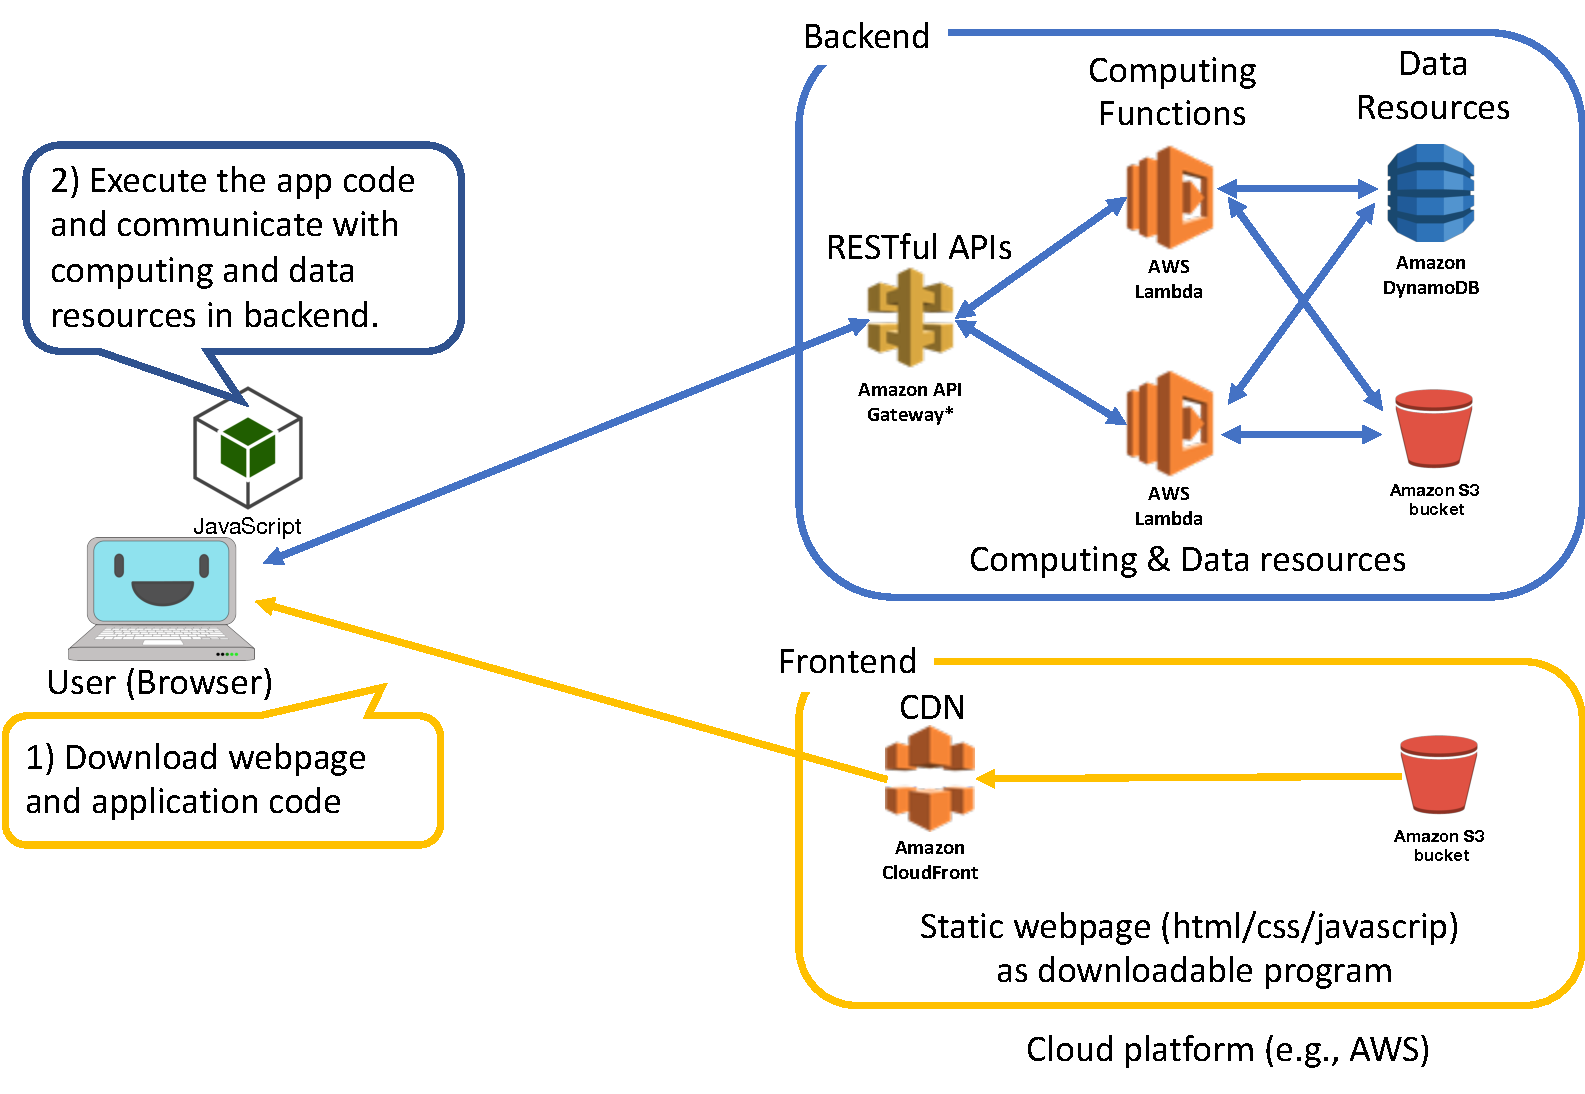
\includegraphics[width=0.85\linewidth]{Figs/spa1.pdf}
\end{center}
\end{frame}

\begin{frame}
AWSを例にした典型的な構成:
\begin{center}
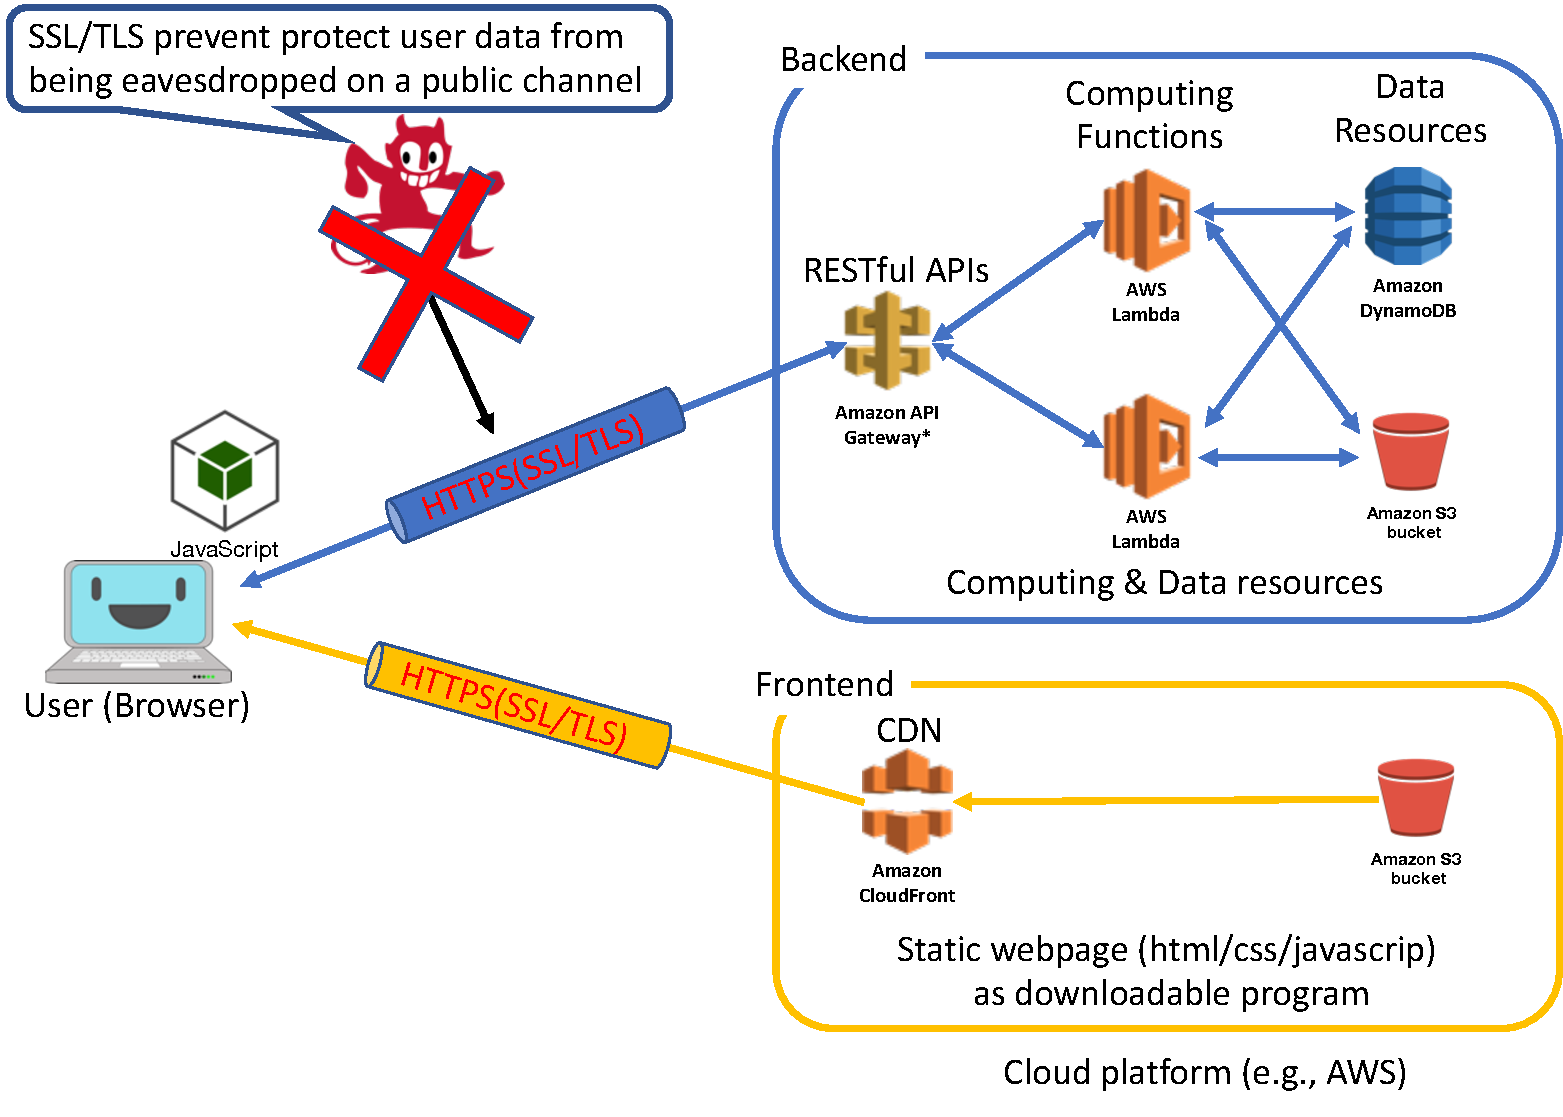
\includegraphics[width=0.85\linewidth]{Figs/spa2.pdf}
\end{center}
\structure{通常、ユーザ・クラウド間のHTTP通信路はSSL/TLSで保護}\\
$\Rightarrow$ HTTP通信路から外部の盗聴者へのユーザデータ漏洩を防止
\end{frame}

\begin{frame}
AWSを例にした典型的な構成:
\begin{center}
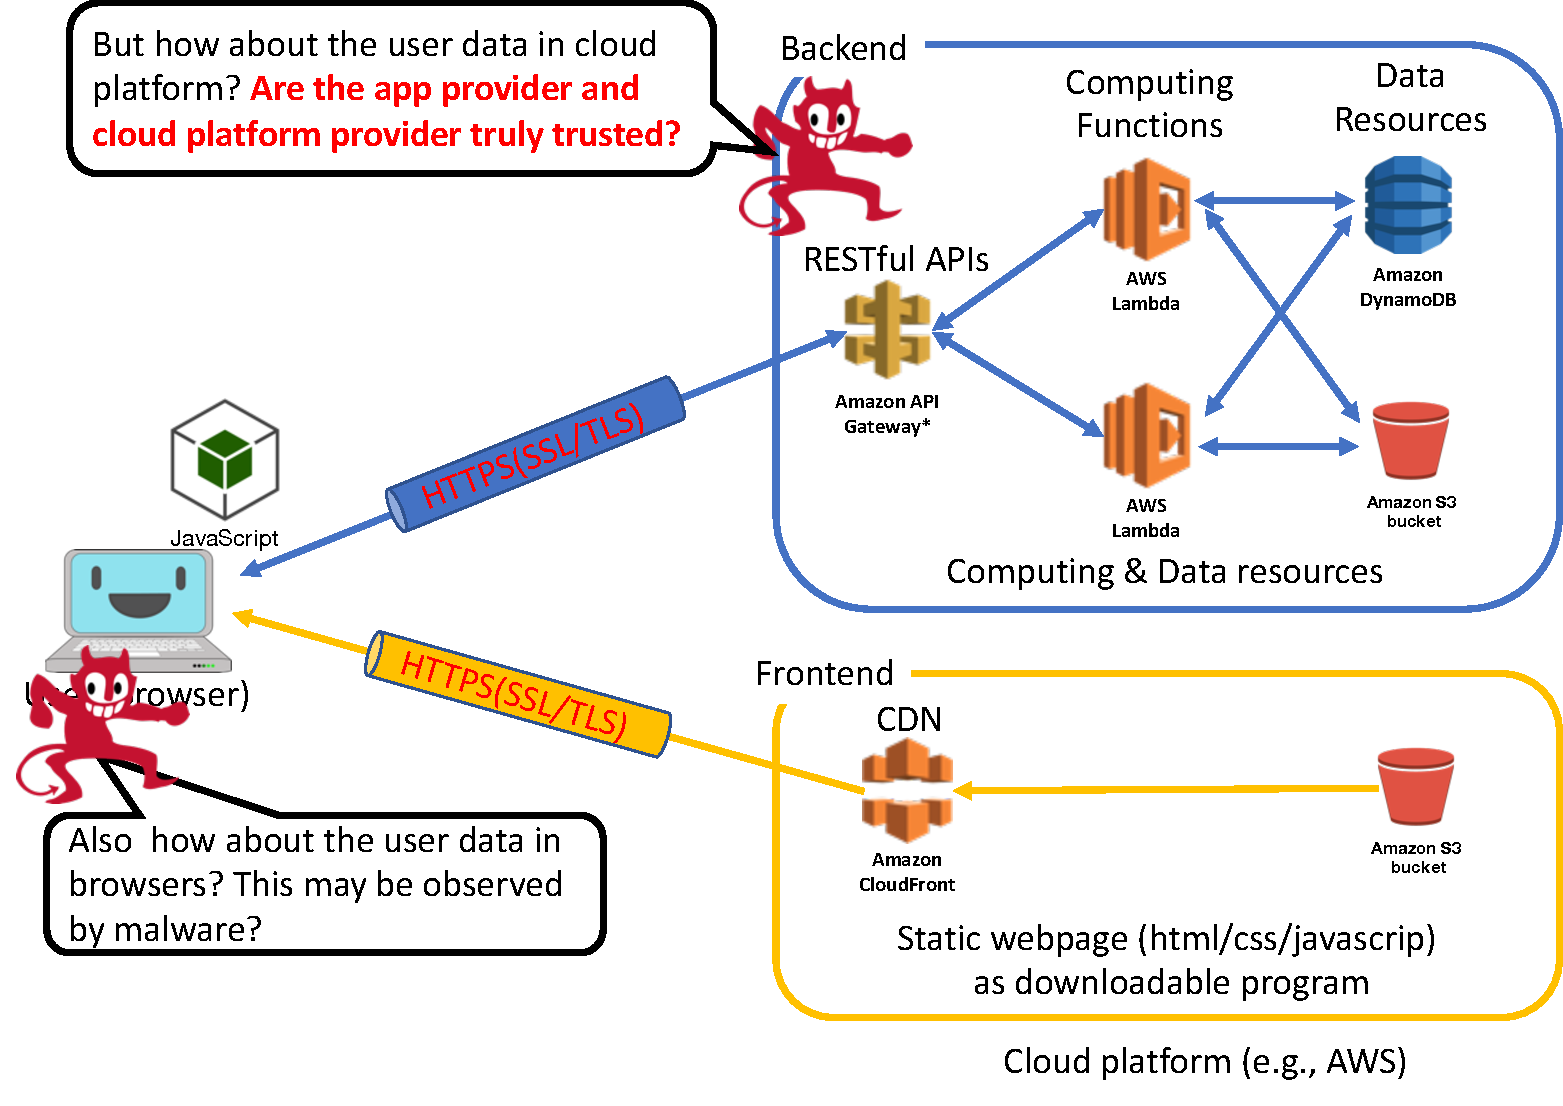
\includegraphics[width=0.85\linewidth]{Figs/spa3.pdf}
\end{center}
\structure{しかし、クラウドPF内・ブラウザ内のデータ保護は……?}
\end{frame}


\begin{frame}
\frametitle{「暗号化しているから安全です」という叙述トリック}

\begin{block}{\small (Webとはちょっと違いますが…)某クラウドストレージ事業者の例}
\begin{center}
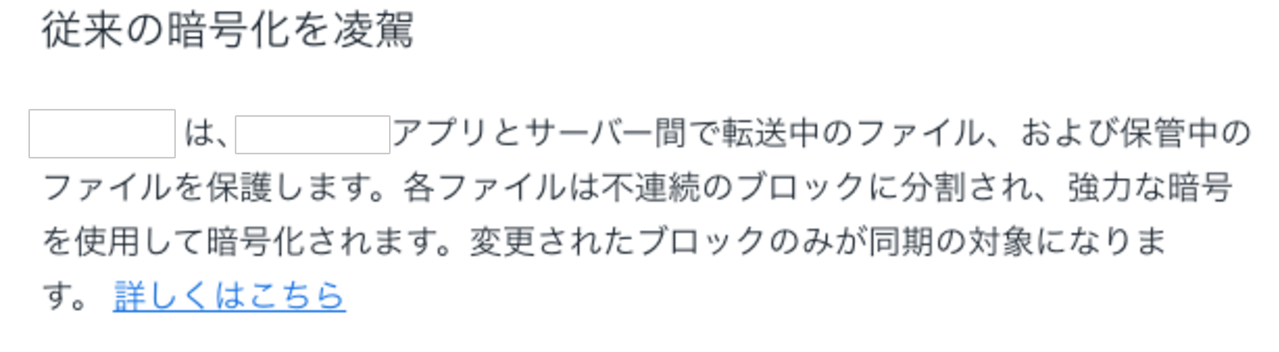
\includegraphics[width=0.8\linewidth]{Figs/storage_enc.pdf}
\end{center} 
\end{block}

クラウドベースの(Web)サービスでよくある文言:
\begin{itemize}
 \item (SSL/TLSで)転送中のデータを暗号化して保護
 \item ストレージに保存されるデータは暗号化して保護
\end{itemize}
\end{frame}

\begin{frame}
\begin{itemize}
 \item (SSL/TLSで)転送中のデータを暗号化して保護\\
 $\Rightarrow$ 公開通信路の盗聴からデータを保護
 \item ストレージに保存されるデータを暗号化して保護\\
 $\Rightarrow$ ストレージ自体が盗まれた時や、第三者のストレージを使っている場合のデータ漏洩を防止%\footnote[frame]{\scriptsize 自社オンプレのストレージサーバを使っている場合、ディスク暗号化する理由が不明。オンプレストレージが盗まれるのか?}
\end{itemize}
\begin{center}
 \structure{いずれも事業者に対しての秘匿性を担保しているわけではない}\footnote[frame]{事業者はデータを見放題ということ。}\\
 $\Downarrow$\\
 \alert{(望む・望まないにしろ)事業者はユーザデータを不必要に取得}
\end{center}
\end{frame}

\begin{frame}
このようなクラウドサービス・Web Appを作ることは:

\begin{itemize}
\item ユーザにとって:共有不要な相手とデータを共有している
\item 事業者にとって:昨今のプライバシ・セキュリティ要求の高まりから、\alert{無用なリスクを背負いこむ可能性が大}
\end{itemize}

\begin{alertblock}{\small 今後、Web Appを作っていくにあたって}
「必要な相手とだけ」確実に・正しく、データを共有できるように、適切なデータ秘匿が必要 (不必要にデータ取得しない)
\end{alertblock}
\end{frame}

\begin{frame}
\frametitle{データの秘匿性・プライバシを謳うサービス}
\small 
\begin{itemize}
\item Tresorit\footnote[frame]{\scriptsize \url{https://tresorit.com/}}:\\
事業者・サーバに情報が漏れないことを謳ったクラウドストレージサービス。Dropboxに近い。

\item KeyBase\footnote[frame]{\scriptsize \url{https://keybase.io/}}:\\
事業者・サーバに情報を漏らさず、メッセージ・ファイル共有(クラウドストレージ)が可能なSNS。

\item Signal\footnote[frame]{\scriptsize \url{https://signal.org/}}:\\
事業者・サーバに情報を漏らさないメッセージング・通話アプリケーション。「最も安全な」チャットサービスと呼ばれており、各類似サービス(WhatsAppなど)にプロトコルを提供。
\end{itemize}

北米・EU共に、スノーデンの事件以降、事業者にも情報を与えない\alert{End-to-End暗号化}を謳ったサービスが強く注目を浴びている。
\end{frame}

\begin{frame}
\frametitle{End-to-Endセキュリティとは}
\begin{block}{End-to-End (E2E) Principle\footnote[frame]{\scriptsize J.~H.~Saltzer et al.\@, ``End-to-End Arguments in System Design'', in Proc. ICDCS 1981, pp. 509--512, Apr. 1981.}}
The end-to-end principle is a network design method in which \alert{application-specific features are kept at communication end points}.\\[1ex]
(アプリケーションの機能はネットワークシステムの\alert{終端}で実装されるべきという原則)
\end{block}
\end{frame}

\begin{frame}
アプリケーションのセキュリティについてのE2E Principle:
\begin{block}{End-to-End (E2E) セキュリティ}
情報を共有する主体同士(End-to-End)について、セキュリティ3原則を担保する。
\begin{itemize}
 \item 情報の秘匿性 (主体のみで情報を共有可能) $\Rightarrow$ \alert{E2E暗号化}
 \item 主体・情報の真正性 (主体が生成した情報であることを証明)
 \item 情報の可用性 (主体同士が正しく情報を利用可能)
\end{itemize}
\end{block}

\end{frame}

\begin{frame}
ポイント:アプリケーションにおいて「情報を共有する主体」は一体何か。
\begin{itemize}
 \item アプリケーションを利用するユーザ同士?
 \item サーバ・クライアントアプリ同士?
 \item 他?
\end{itemize}
\end{frame}

\begin{frame}
では、Webアプリケーションにおけるエンドポイントとは?
\begin{itemize}
\item ユーザ側エンド:\\
 $\Rightarrow$ \alert{JavaScript/HTML/CSSなど「ブラウザ内で実行・レンダリングされる」Webフロントエンド要素}\footnote[frame]{\scriptsize 実際にユーザが触れる要素がエンドポイントであって、\alert{Webサービスにおいては、端末やブラウザはエンドポイントにならない}}\\
\item もう一方のエンド:\\
 $\Rightarrow$ \structure{Webアプリケーション次第で変化}
\end{itemize}

\end{frame}


\begin{frame}
例: クラウドプラットフォームを介し、\alert{ユーザ同士が情報を共有する主体}の場合 = ユーザのブラウザ同士が両エンド
\begin{center}
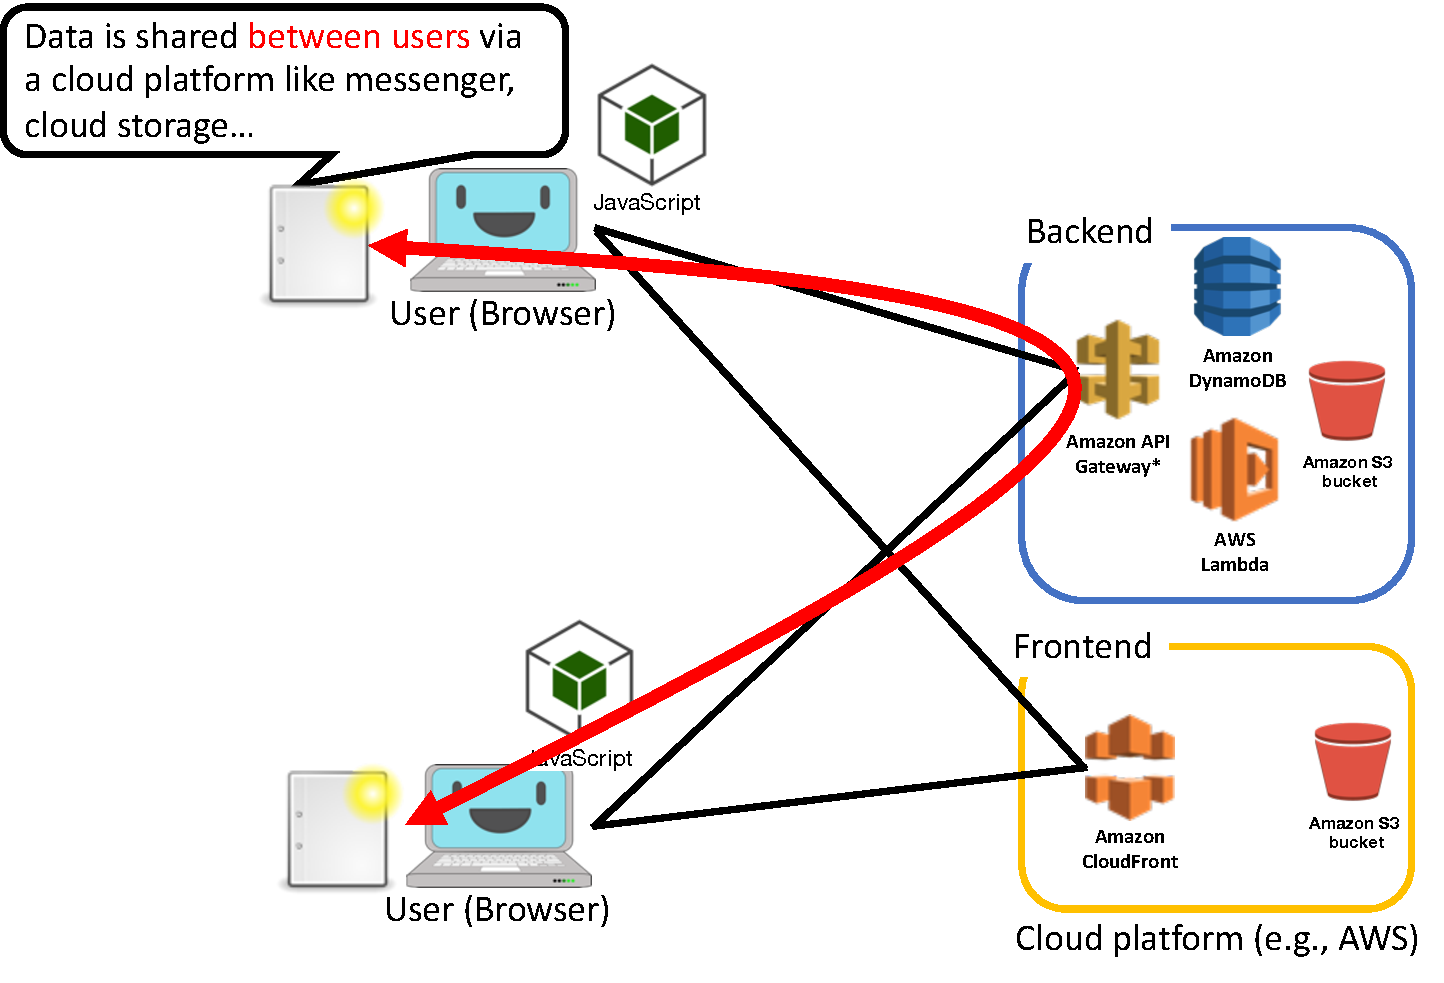
\includegraphics[width=0.8\linewidth]{Figs/e2e1.pdf}
\end{center}
\end{frame}

\begin{frame}
E2Eセキュリティの観点からは、\alert{クラウドプラットフォーム自身ですら情報を取得可能であるべきではない}
\begin{center}
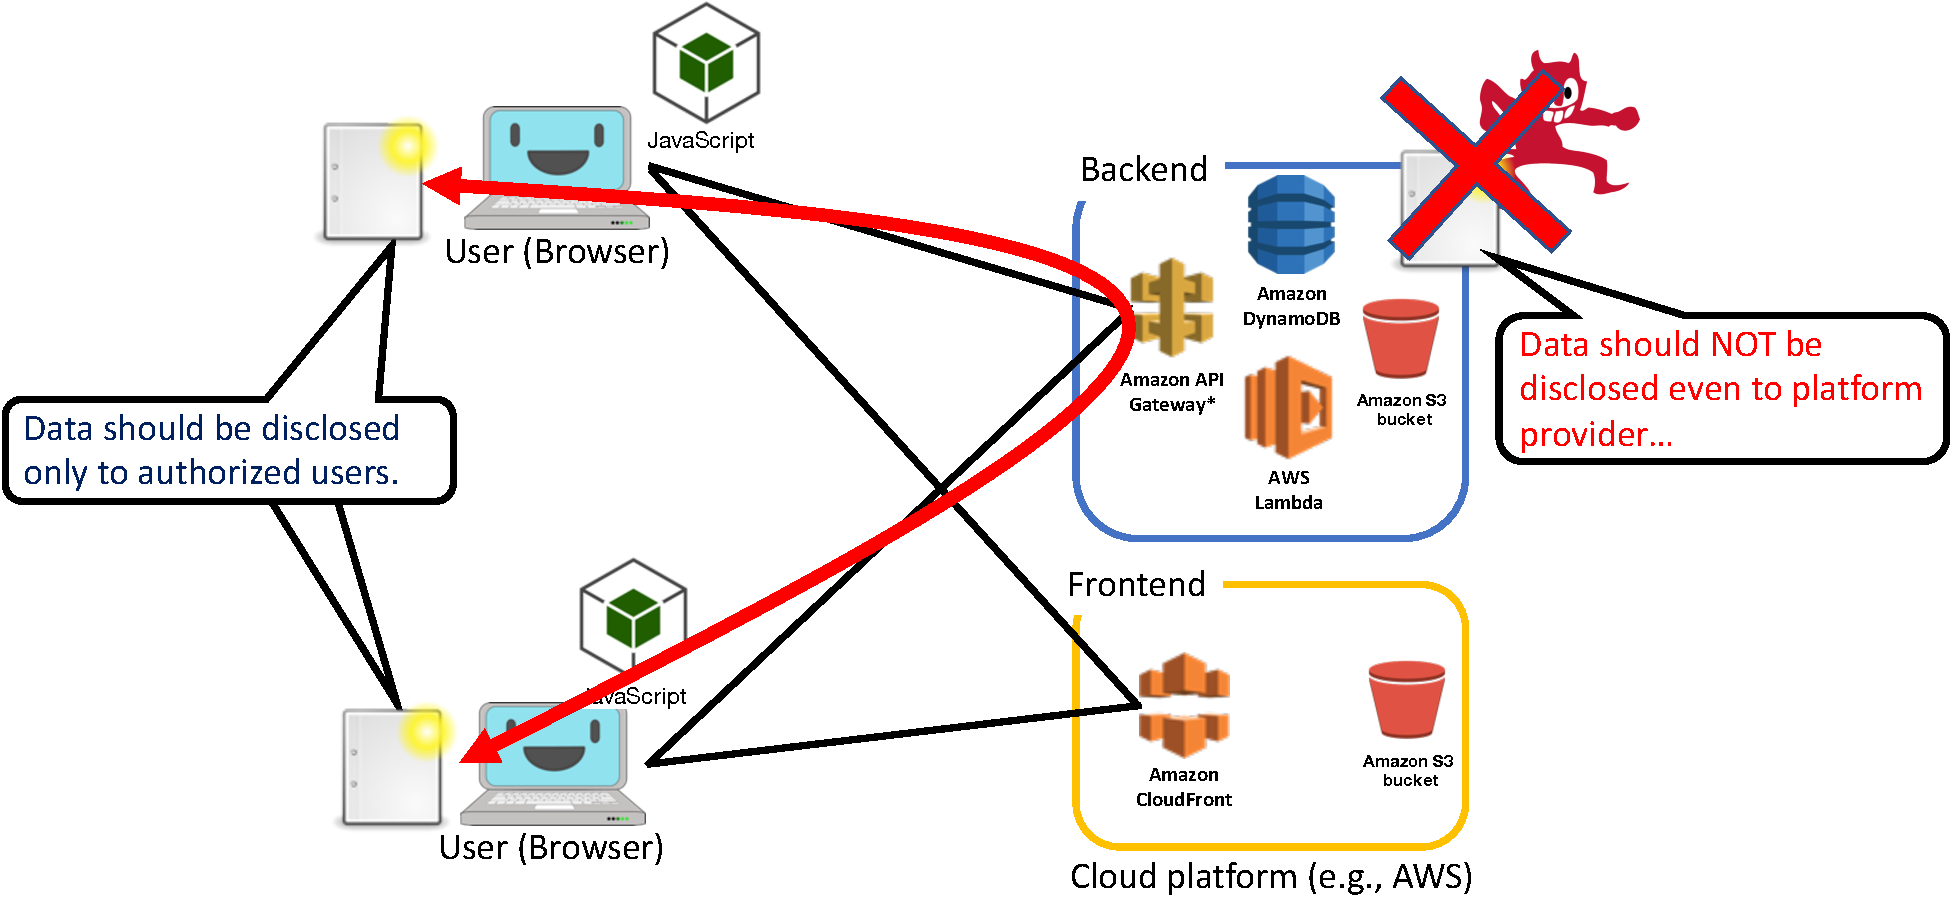
\includegraphics[width=\linewidth]{Figs/e2e2.pdf}
\end{center}
{\footnotesize ※ユーザがサーバとのみやり取りする場合、一方の主体(End)はサーバとなる。}
\end{frame}

\begin{frame}
この例の場合、E2Eセキュリティのためには、
情報を共有する主体同士のみが復号可能なよう、やり取りするデータを全て暗号化する (\alert{E2E暗号化})
\begin{center}
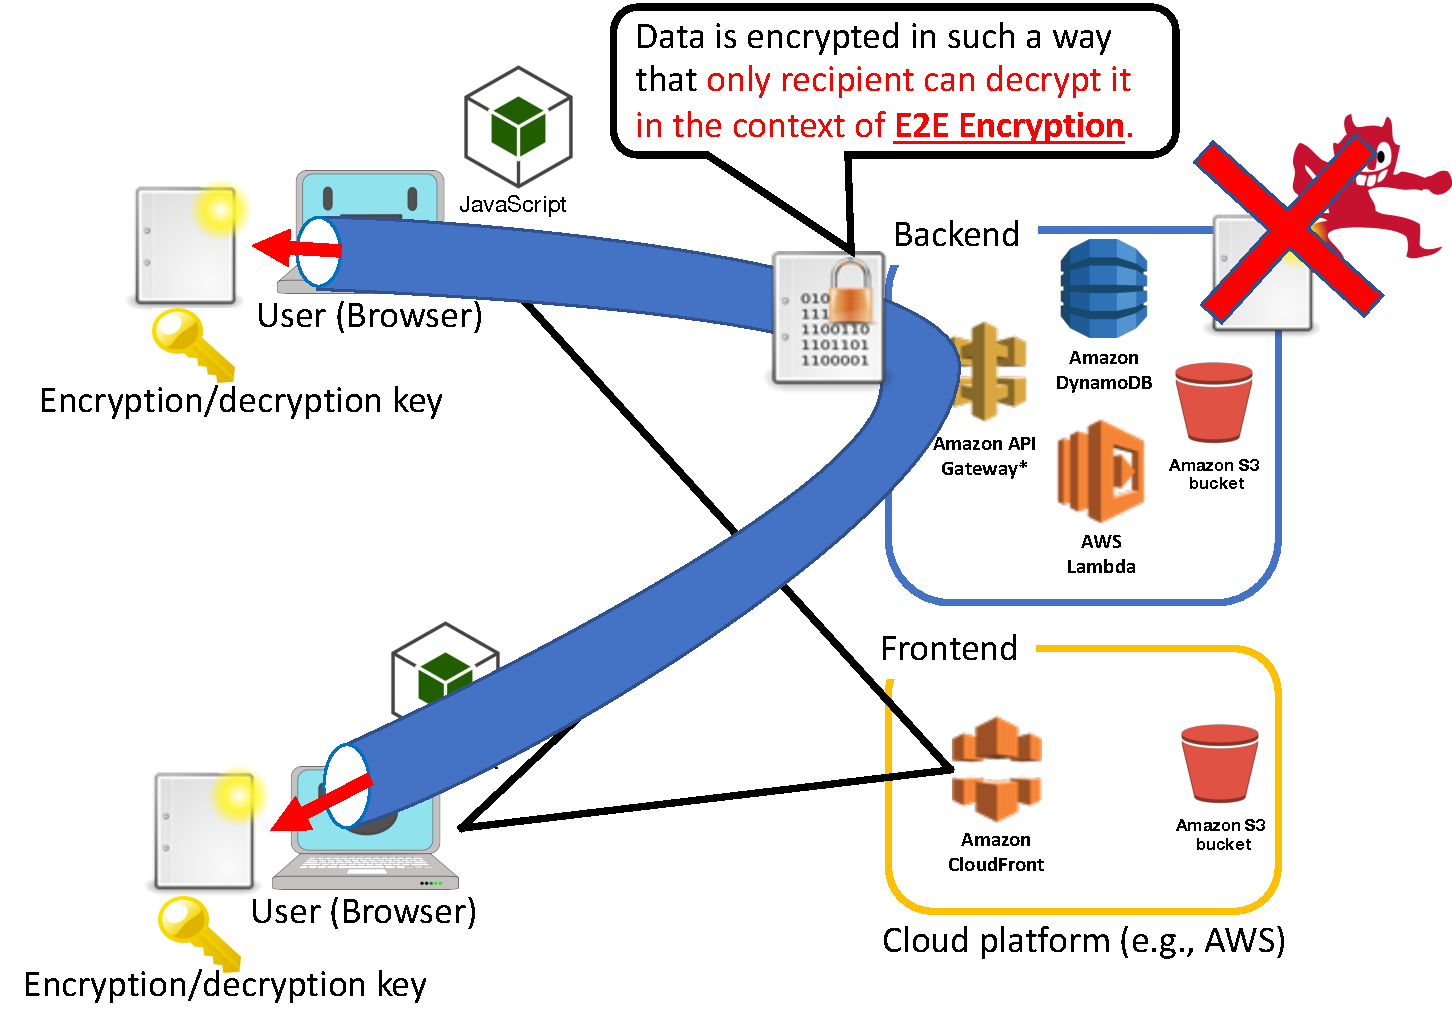
\includegraphics[width=0.8\linewidth]{Figs/e2e3.pdf}
\end{center}
\end{frame}

\begin{frame}
\begin{alertblock}{}
E2Eセキュリティを実現するには、\structure{構築するアプリケーション毎に「情報を共有する主体」を正しく定義}する必要。
\end{alertblock}

E2Eセキュリティを実現しつつ、「事業者にとってリスクとなるような情報はなるべく不用意に取得しない」ことも重要。
\end{frame}

\begin{frame}
\frametitle{Web AppにおけるEnd-to-Endセキュリティ}
改めて…
\begin{block}{\small サービスでE2Eセキュリティを考える意味}
\begin{itemize}
 \item ユーザプライバシの保護
 \item 事業者側のリスクの低減
\end{itemize}
\end{block}

\begin{exampleblock}{\small WebアプリケーションにおけるE2Eセキュリティ}
少なくとも片方のエンドはWebフロントエンド要素\\
$\Rightarrow$ \alert{Webフロントエンドでセキュリティを担保する方法が必要}
\end{exampleblock}

\end{frame}

\begin{frame}
と、いうわけで、今回は「WebのためのE2Eセキュリティ」としてJavaScriptにおけるデータの暗号化(E2E暗号化)の「さわり」を紹介します。
\end{frame}

%%%%%%%%%%%%%%%%%%%%%%%%%%%%%%%%%%%%%%%%%%%%%%%%%%%%%%%%%%%%%%%%%%%%%%%%%%%%%%%%%%%%%%%%%%%%%%%%%%%
\section{JavaScriptで暗号を使ってみよう [基礎編]}

\subsection{導入}
\begin{frame}
\centering
{\Large JavaScriptで暗号を使ってみよう [基礎編]}

\vspace{1ex}
--今回はお試しでAES--

\end{frame}

\begin{frame}
\frametitle{AES (Advanced Encryption Standard) とは?}
\begin{block}{AES}
米国NISTの標準暗号アルゴリズム (※共通鍵暗号)\\
\begin{itemize}
 \item 鍵長は3種類: 128-bit, 192-bit, 256-bit
 \item 欧州NESSIE、日本CRYPTRECなどの標準規格としても採択
 \item 現在まで致命的な欠陥は見つかっていない、安全性の高い\alert{デファクトスタンダード}のアルゴリズム
\end{itemize}
\end{block}
\begin{center}
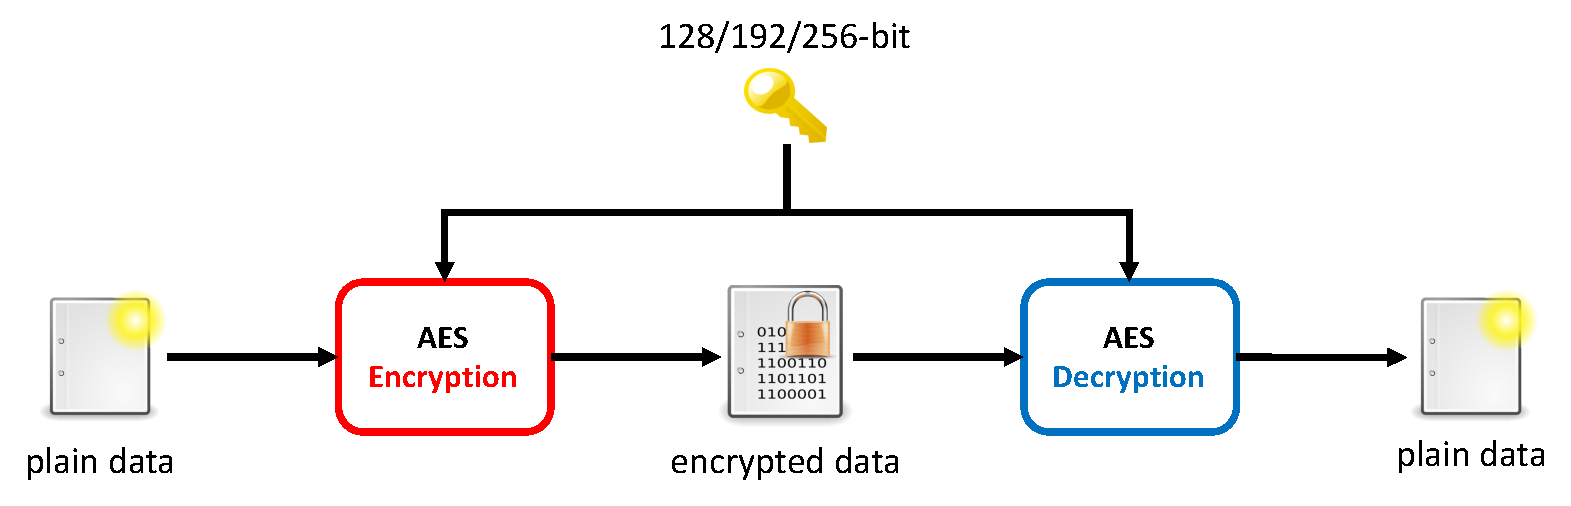
\includegraphics[width=0.9\linewidth]{Figs/aes_flow.pdf}
\end{center}
\end{frame}

\begin{frame}
共通鍵暗号・公開鍵暗号・ハッシュがどうのとか、それらを組み合わせて安全に使うためにはどうするかとか、そういう話は今回はしない。

\vspace{1ex}

とりあえず「AESという暗号アルゴリズムがあるんだ」くらいで十分。
今回、まずは「\alert{とにかくJSでAESを使ってデータを暗号化してみること}」から始める。
\end{frame}


\begin{frame}
\frametitle{JavaScriptにおける暗号の利用環境}
\small
一般的な統合ライブラリはCで書かれたOpenSSLだが、
JavaScriptから直接呼び出すことができない。

\vspace{1ex}

JavaScriptから利用可能な暗号の統合ライブラリ:
\begin{itemize}
\item \alert{\texttt{WebCrypto API}} (ブラウザ)\footnote[frame]{\url{https://www.w3.org/TR/WebCryptoAPI/}}:\\
W3Cにて標準化が進むWeb API (ブラウザのネイティブAPI)。
\item \alert{\texttt{Crypto}} (Node.js)\footnote[frame]{\url{https://nodejs.org/api/crypto.html}}:\\
Node.js環境にて利用可能な暗号ライブラリ (Node.jsのネイティブAPI)。OpenSSLのラッパー。
\item \texttt{sjcl} (Node.js/ブラウザ)\footnote[frame]{\url{http://bitwiseshiftleft.github.io/sjcl/}}:\\
Stanford大学暗号研究室で開発されたpure JSなライブラリ。
\end{itemize}
\end{frame}

\begin{frame}
今回は、高速動作が期待されるネイティブ実装な統合ライブラリ2つを例にとる。
\begin{itemize}
 \item WebCrypto API → ブラウザ向け
 \item Node Crypto → サーバ/スタンドアロンS/W (Node.js) 向け
\end{itemize}
\end{frame}

\begin{frame}
\frametitle{今回やってみること}
ブラウザ・Node.jsをエンドとし、REST APIで暗号化データを登録してみる。
\begin{center}
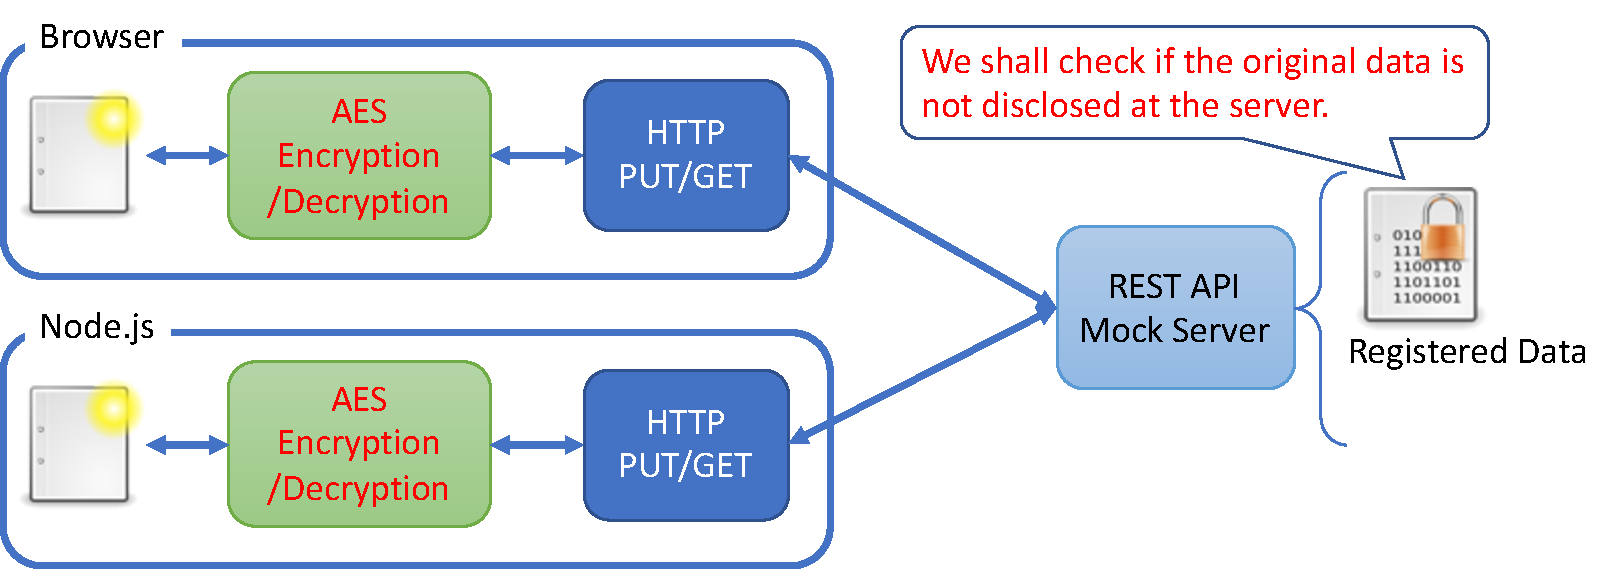
\includegraphics[width=\linewidth]{Figs/mock_flow.pdf}
\end{center}
単なるデータのHTTP PUT/GETの前段・後段にAES暗号化・復号部分を組み込んでみる。

※モックサーバはローカルホストで立ち上げ。
\end{frame}

\begin{frame}
\frametitle{環境}
以下の環境が前提:
\begin{itemize}
 \item Node.js ($>$ v10)がインストール済 \footnote[frame]{npmに加えてyarnも使えるとなお良い (インストールコマンド: npm i -g yarn)}
 \item ブラウザとして、Google Chrome (系ブラウザ)、もしくはFirefoxがインストール済み
 \item Visual Studio Code や WebStorm などの統合開発環境がセットアップ済みだとなお良い。
\end{itemize}
\end{frame}

\begin{frame}
\frametitle{JavaScriptプロジェクトの準備}
\begin{itemize}
\item プロジェクトのGitHubリポジトリ\footnote[frame]{\url{https://github.com/zettant/e2e-security-01}}をClone\\
\begin{exampleblock}{}
\footnotesize
\$ \texttt{git clone https://github.com/zettant/e2e-security-01}\\
\$ \texttt{cd e2e-security-class/sample}
\end{exampleblock}
\item 依存パッケージのインストール
\begin{exampleblock}{}
\$ \texttt{yarn install}\quad or\quad \texttt{npm install}
\end{exampleblock}
\item ライブラリのビルド
\begin{exampleblock}{}
\$ \texttt{yarn build}\quad or\quad \texttt{npm run build}
\end{exampleblock}
\end{itemize}
\end{frame}

\begin{frame}
\frametitle{REST APIモックサーバの準備}
今回はSSL接続可能な共有サーバを準備済 (\url{https://e2e.zettant.com/})。

\vspace{2ex}

別途、検証用のサーバをローカルで立ち上げ可能。
\begin{exampleblock}{\small モックサーバの立ち上げ}
\$ \texttt{yarn start}
\end{exampleblock}
起動すると、localhostの3000番ポートでHTTPリクエストを待ち受け開始する。
\end{frame}


\subsection{とりあえず試してみる: コマンドライン編}
\begin{frame}
\centering
{\Large とりあえず試してみる: コマンドライン編}
\end{frame}

\begin{frame}
\frametitle{とりあえず試してみる: コマンドライン編}
JavaScript (Node.js) をコマンドラインから実行してみて、動作イメージを確認してみる。
\begin{center}
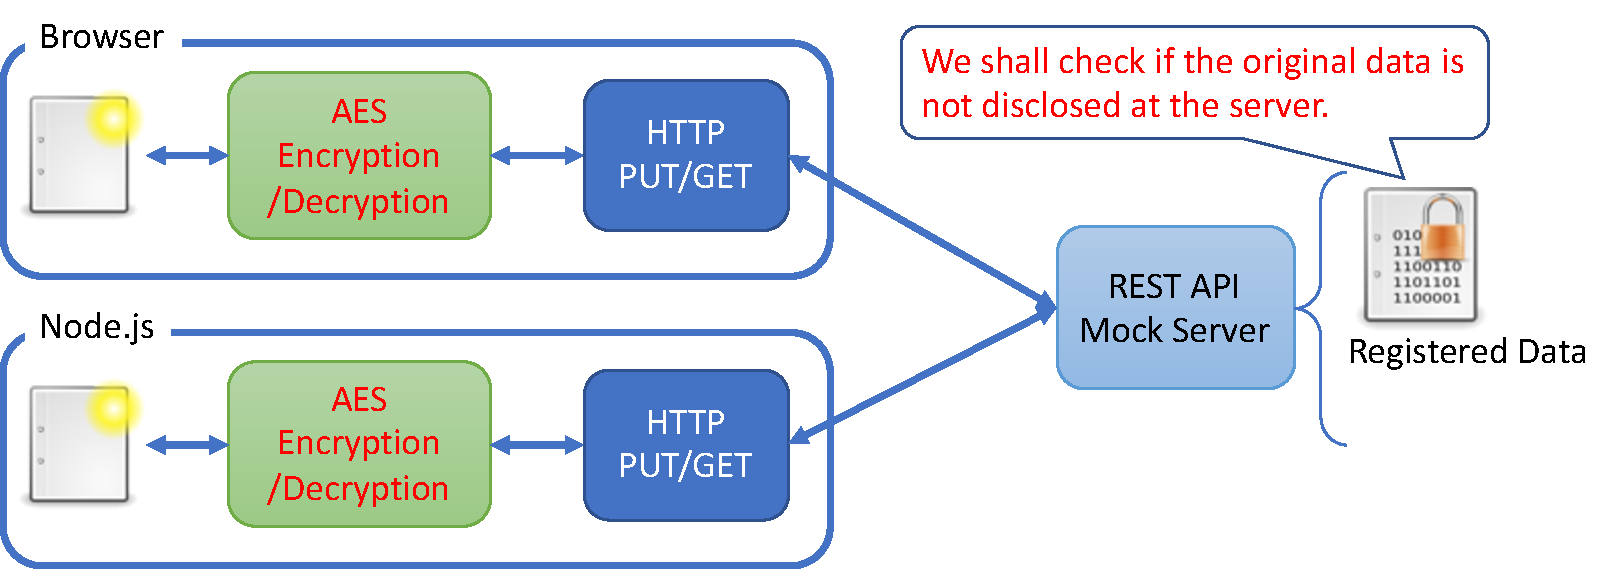
\includegraphics[width=\linewidth]{Figs/mock_flow.pdf}
\end{center}
\end{frame}

\begin{frame}
まずは生データをPOSTしてサーバに登録してみる。
\begin{exampleblock}{}\footnotesize
\$ \texttt{pwd}\\
\texttt{.../e2e-security-class/sample} ←場所を確認\\[1ex]
\$ \texttt{yarn execute post -r 'hello my secret world!!!'} ← \alert{登録}\footnote[frame]{\texttt{-r}を抜くとローカルのモックサーバに接続}\\
\texttt{Register plaintext data to remote server}\\
\texttt{Data: hello my secret world!!!}\\
\textbf{\texttt{Registered id: 1}} ←\alert{id=1番として登録したというメッセージ}
\end{exampleblock}

登録したデータを生のまま取得してみる。
\begin{exampleblock}{}\footnotesize
\$ \texttt{yarn execute get -r 1} ← \alert{id=1番の登録データを取得}\\
\texttt{Retrieve plaintext data to remote server}\\
\texttt{Registered Id: 1}\\
\textbf{\texttt{Retrieved data: hello my secret world!!!}} ← \alert{取得した1番のデータ}
\end{exampleblock}
\end{frame}



\begin{frame}
データをAES暗号化したあとPOSTしてサーバに登録してみる。
\begin{exampleblock}{}\footnotesize
\$ \texttt{yarn execute post $\backslash$}\\
~ \textbf{\texttt{-e -k 'my secret key' $\backslash$}} ← \alert{\texttt{my secret key}という鍵で暗号化}\\
~ \texttt{-r 'hello my super secret world!!!'}\\
\texttt{Register encrypted data to remote server}\\
\texttt{Data: hello my super secret world!!!}\\
\texttt{Key: my secret key}\\
\texttt{Note: Derived key binary in base64: o12da4tawTjHd4woS+DeexcCR9EOyVKml6gOzZkGzDc=}\footnote[frame]{実際に使うAES鍵のバイナリ表現 (base64)}\\
\textbf{\texttt{Registered id: 2}} ←\alert{id=2番として登録したというメッセージ}
\end{exampleblock}

\end{frame}

\begin{frame}
暗号化して登録したデータを生のまま取得してみて、暗号化されていることを確認する。
\begin{exampleblock}{}\footnotesize
\$ \texttt{yarn execute get -r 2} ← \alert{id=2番の登録データを取得}\\
\texttt{Retrieve plaintext data to remote server}\\
\texttt{Registered Id: 2}\\
\textbf{\texttt{Retrieved data: EoeSsv5BFr6s1jZh3iMM1Pxa+wA4UxQnM30J2027kJU=}} ← \alert{取得した2番のデータ}
\end{exampleblock}
Base64エンコードされているが、暗号化されており中身はまったくわからない。\footnote[frame]{Mac/Linuxの場合、ターミナルで``\texttt{echo [base64str] $\mid$ base64 -D -}'' と実行してみると訳のわからないデータにデコードされることが確認できる。}
\end{frame}

\begin{frame}
取得した後、復号してみる\footnote[frame]{keyが間違っていると失敗する}
\begin{exampleblock}{}\footnotesize
\$ \texttt{yarn execute get $\backslash$}\\
~ \textbf{\texttt{-d -k 'my secret key' $\backslash$}} ←\alert{my secret keyという鍵で復号}\\
~ \texttt{-r 2} ← id=2の鍵を取得\\
\texttt{Retrieve encrypted data to remote server}\\
\texttt{Id: 2}\\
\texttt{Key: my secret key}\\
\texttt{Note: Derived key binary in base64: o12da4tawTjHd4woS+DeexcCR9EOyVKml6gOzZkGzDc=}\\
\textbf{\texttt{Decrypted data: hello my super secret world!!!}} ←\alert{正しく復号された}
\end{exampleblock}
\end{frame}

\begin{frame}
\url{https://e2e.zettant.com/data} にアクセスすると、サーバでの登録状況が一覧できる。\footnote[frame]{ローカルホストに立てた場合は\url{http://localhost:3000/data}}

\begin{center}
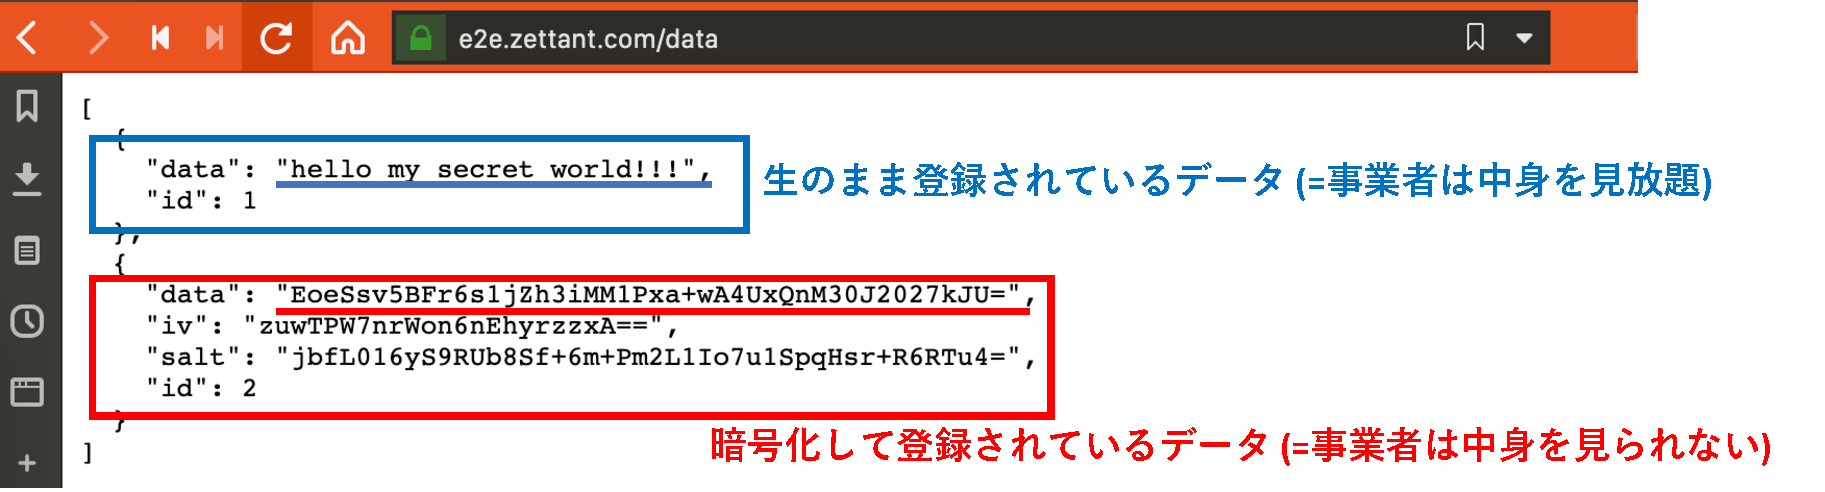
\includegraphics[width=\linewidth]{Figs/json_list.pdf}
\end{center}
\end{frame}

\subsection{とりあえず試してみる: ブラウザ編}
\begin{frame}
\centering
{\Large とりあえず試してみる: ブラウザ編}
\end{frame}

\begin{frame}
\frametitle{とりあえず試してみる: ブラウザ編}
\begin{enumerate}
 \item \texttt{samples/src/post-get-browser.html}をブラウザで開く。
 \item 真っ白な画面で「開発者ツール」を起動\footnote[frame]{Chrome: Ctrl(Cmd)+Alt(Opt)+i}、Webコンソールを表示する。
\end{enumerate}

コマンドラインでやった「暗号化して登録→取得して復号」の一連の流れが初期設定のデータ・鍵を使って実行される。

\begin{center}
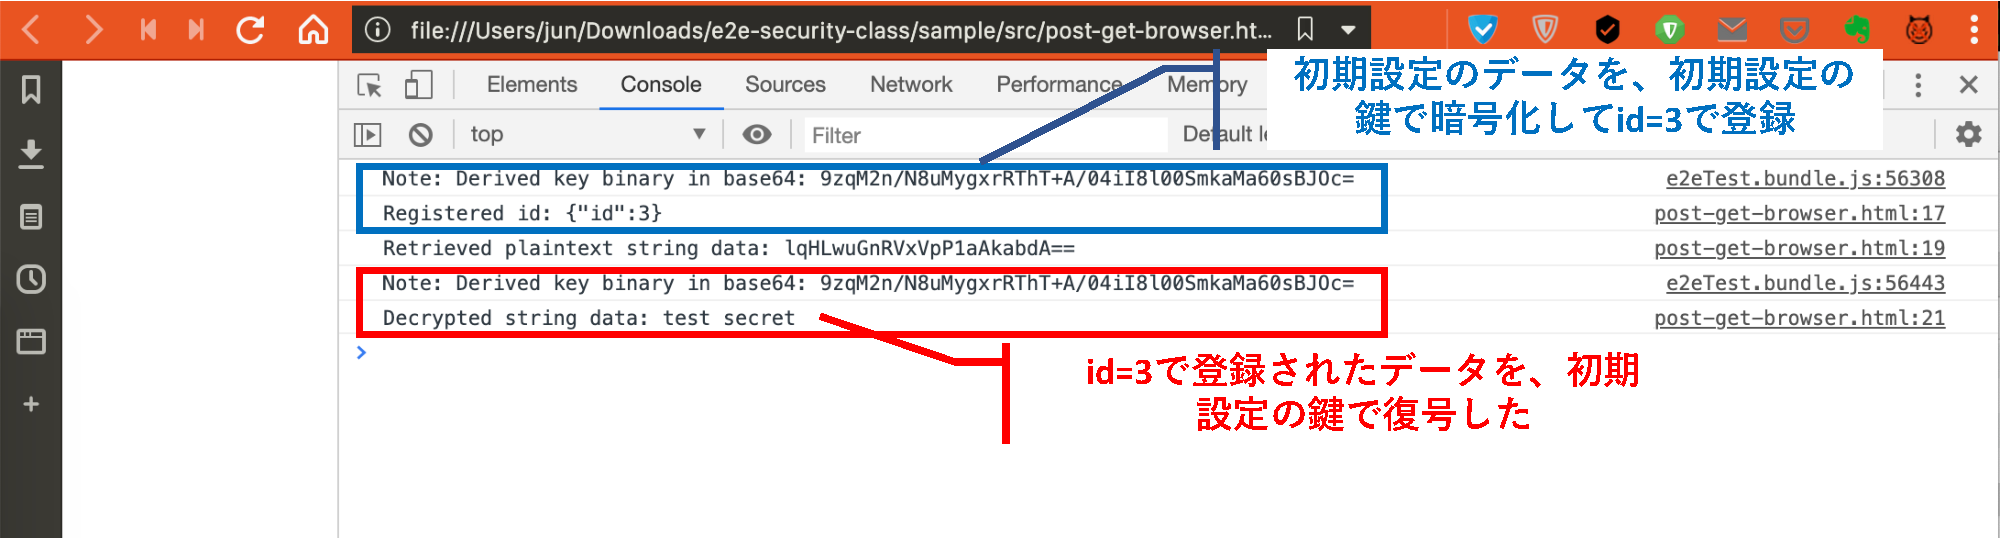
\includegraphics[width=\linewidth]{Figs/browser-img1.pdf}
\end{center}

\end{frame}

\begin{frame}
以下の2パターンで色々試すことができる。
\begin{itemize}
 \item \texttt{samples/src/post-get-browser.html}の中身を編集→リロード
 \item \texttt{samples/src/post-get-browser.html}を開いたまま、開発者ツールのWebコンソールからPOST関数とGET関数を実行。
\end{itemize}
ここでは後者を試してみる。
\end{frame}

\begin{frame}[fragile]
Webコンソールから暗号化・登録してみる。
\begin{center}
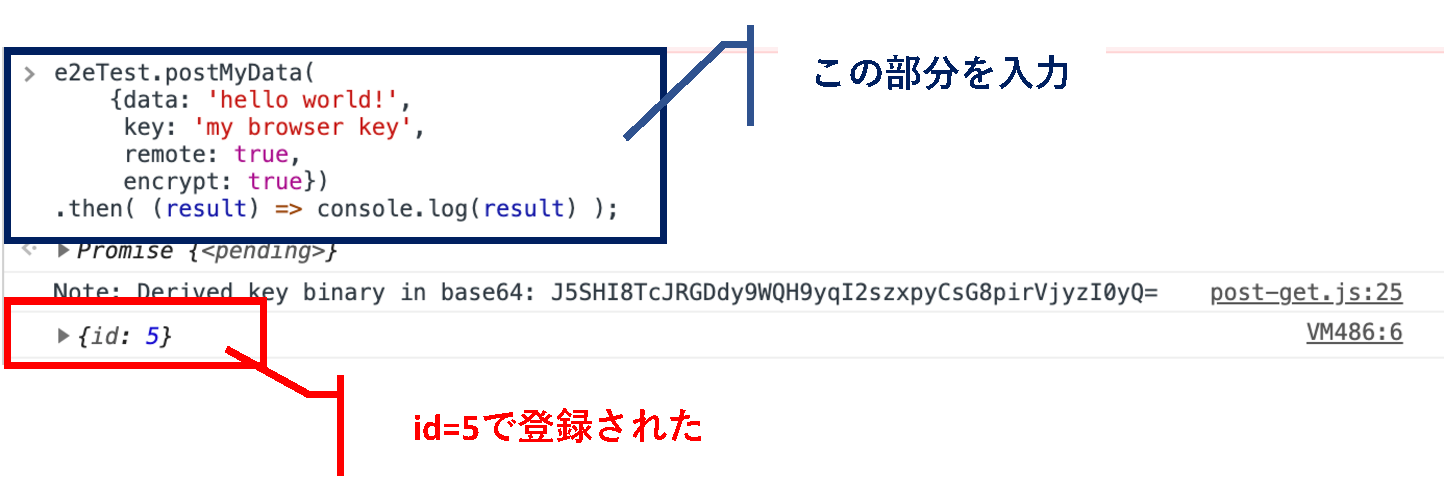
\includegraphics[width=0.9\linewidth]{Figs/browser-img2.pdf}
\end{center}

\begin{exampleblock}{}\footnotesize
\begin{verbatim}
e2eTest.postMyData(
    {data: 'hello world!', ← 暗号化するデータ
     key: 'my browser key', ← 鍵
     remote: true, ← リモートサーバの場合true
     encrypt: true}) ← 暗号化する場合true
.then( (result) => console.log(result) );
\end{verbatim}
〜中略〜\\[1ex]
\textbf{\texttt{VM486:6 \{id: 5\}}}
\end{exampleblock}
\end{frame}

\begin{frame}
 コマンドラインと同じく、\url{https://e2e.zettant.com/data}を表示すると暗号化されて登録されていることがわかる。
\end{frame}

\begin{frame}[fragile]
今度はWebコンソールから取得・復号してみる。
\begin{center}
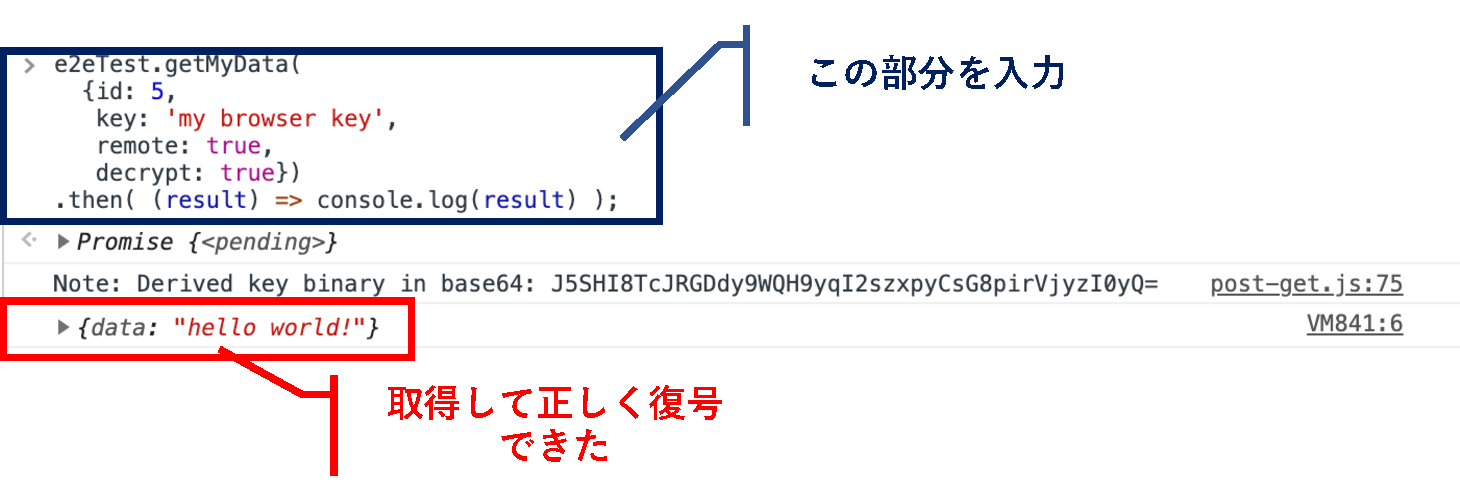
\includegraphics[width=0.9\linewidth]{Figs/browser-img3.pdf}
\end{center}
\begin{exampleblock}{}\footnotesize
\begin{verbatim}
e2eTest.getMyData(
  {id: 5, ← id=5のデータを取得
   key: 'my browser key', ← 鍵
   remote: true, ← リモートサーバの場合true
   decrypt: true}) ← 復号する場合true
.then( (result) => console.log(result) );
\end{verbatim}
〜中略〜\\[1ex]
\textbf{\texttt{{data: "hello world!"}}}
\end{exampleblock}
\end{frame}

\begin{frame}
もちろん、ブラウザ(WebCrypto)とコマンドラインで相互接続可能。
\begin{itemize}
 \item ブラウザで暗号化・登録したデータを、コマンドラインで取得・復号
 \item コマンドラインで暗号化・登録したデータを、ブラウザで取得・復号
\end{itemize}
\begin{center}
今まで登録したデータで試してみよう! 
\end{center}
\end{frame}

\subsection{暗号化・復号の中身}
\begin{frame}
\centering
{\Large 暗号化・復号の中身}
\end{frame}

\begin{frame}
\frametitle{今回の事例でのモード設定}

\begin{block}{\small AESの「利用モード」}
AESの処理1回で暗号化できるのはたった16bytesにすぎない。

長いデータを連続で暗号化するために、\alert{暗号化処理を連続して組み合わせる方法}が利用モード。
\end{block}
\end{frame}

\begin{frame}
安全性向上のため、一般的に
\begin{itemize}
 \item 「先頭の16バイトはランダムな初期化ベクトルと混ぜる」
 \item 「前の16バイトのデータを継承して次の16バイトを処理」
\end{itemize}
などの工夫を入れた利用モードを用いる。

\begin{center}
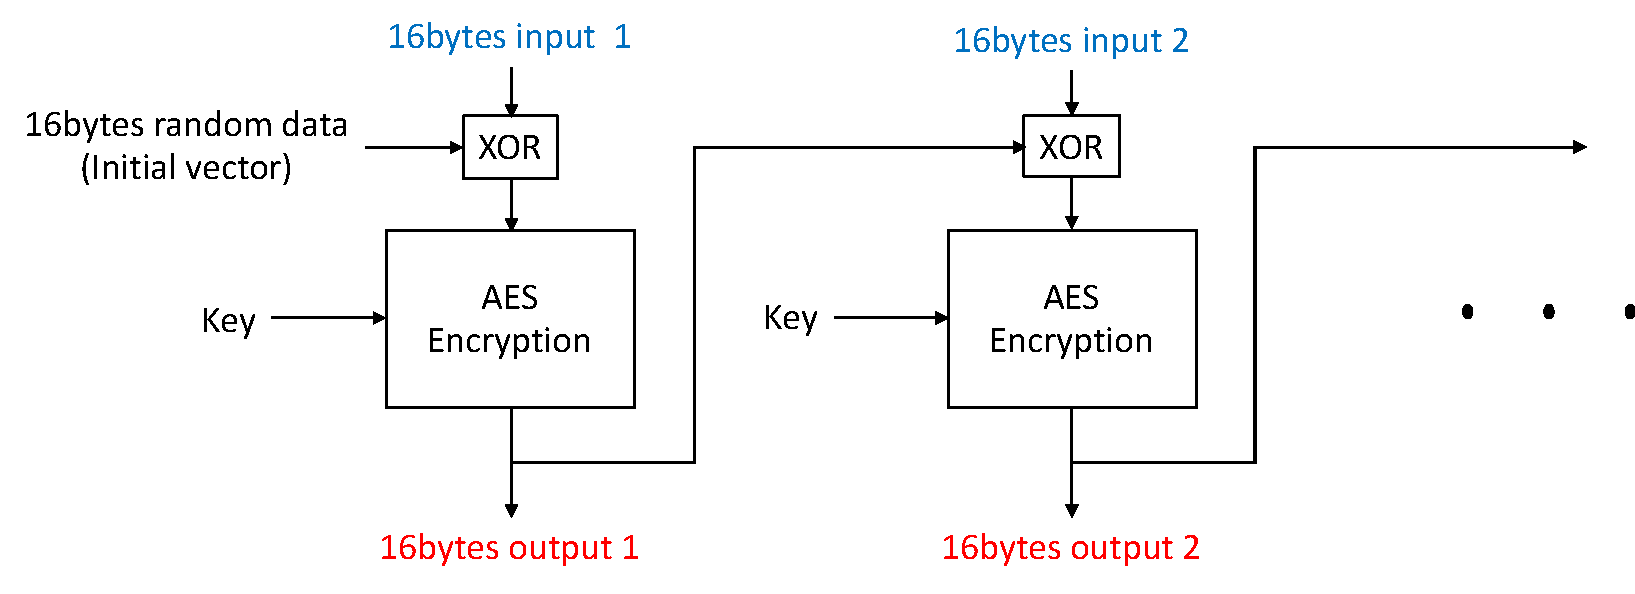
\includegraphics[width=0.8\linewidth]{Figs/cbc_mode.pdf}
\end{center}

\vspace{2ex}
今回の事例では、256ビット鍵AESのCBCモード\footnote[frame]{ISO等で標準化されている一般的に安全なモード}を用いた。
\end{frame}


\begin{frame}[fragile]
\frametitle{Node.js CryptoライブラリでのAES-CBC暗号化・復号}
\begin{block}{\small \texttt{sample/src/encrypt-node.js}: encrypt関数}
\scriptsize
\begin{verbatim}
const crypto = require('crypto'); // cryptoモジュールの読み出し
const algorithm = 'aes-256-cbc'; // AES-256-CBCモード

const iv = crypto.randomBytes(16); // Initial Vectorの生成

const cipher = crypto.createCipheriv(algorithm, key, iv); // 暗号化Object初期化
let encrypted = cipher.update(uint8data, 'utf8', 'base64'); // 暗号化
encrypted += cipher.final('base64'); // 暗号化完了
\end{verbatim}
\end{block}

\begin{center}
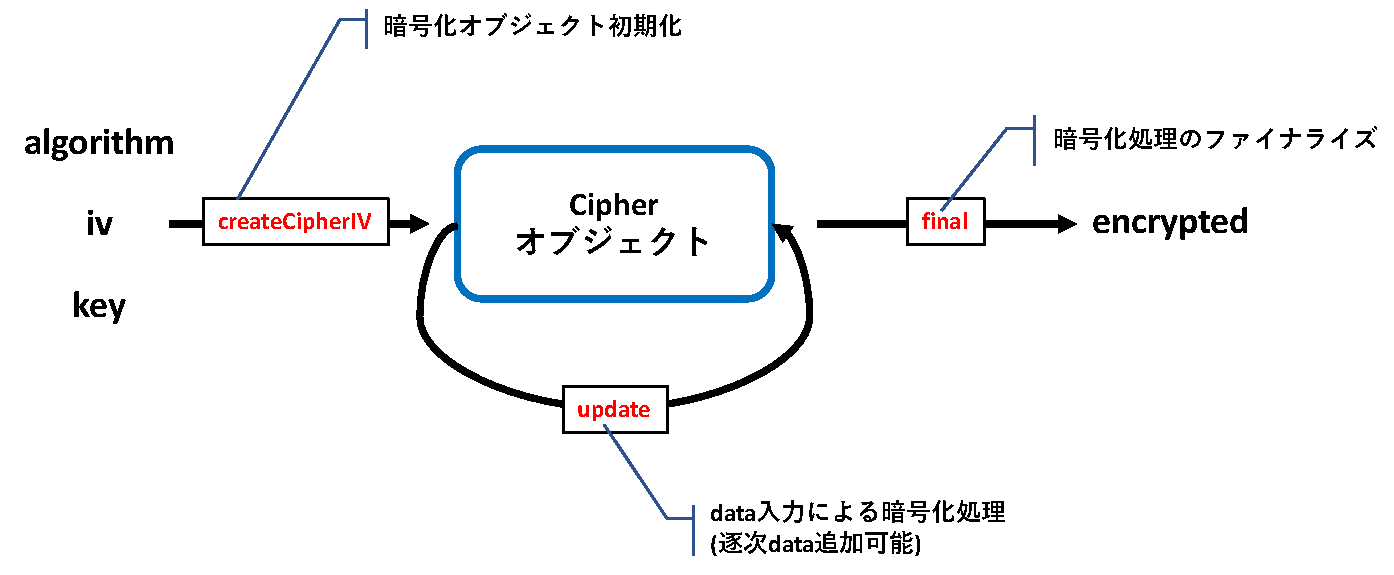
\includegraphics[width=0.8\linewidth]{Figs/node_aes_e.pdf}
\end{center}
\end{frame}

\begin{frame}[fragile]
\scriptsize
\begin{block}{\small \texttt{sample/src/encrypt-node.js}: decrypt関数}
\begin{verbatim}
const crypto = require('crypto'); // cryptoモジュールの読み出し
const algorithm = 'aes-256-cbc'; // AES-256-CBCモード

const decipher = crypto.createDecipheriv(algorithm, key, iv); // 復号Object初期化
let decrypted = decipher.update(encrypted, 'base64', 'utf8'); // 復号
decrypted += decipher.final(); // 復号完了
\end{verbatim}
\end{block}
\begin{center}
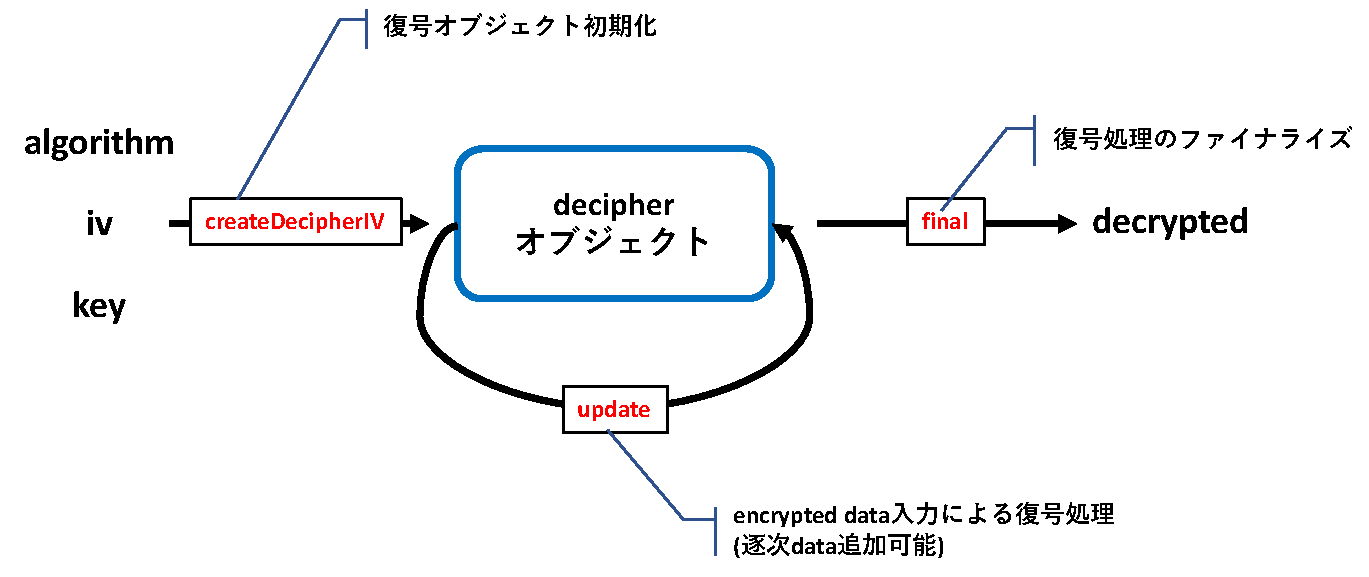
\includegraphics[width=0.8\linewidth]{Figs/node_aes_d.pdf}
\end{center}
\end{frame}


\begin{frame}[fragile]
\frametitle{ブラウザ WebCrypto APIでのAES-CBC暗号化・復号}

\begin{block}{\small \texttt{sample/src/encrypt-browser.js}: encrypt関数}
\scriptsize
\begin{verbatim}
const crypto = window.crypto; // WebCrypto API
const iv = crypto.getRandomValues(new Uint8Array(16)); // IVの生成

const importedKey = await crypto.subtle.importKey( // keyオブジェクトの生成
  'raw', // バイナリ鍵のインポート指定
  key,
  { name: 'AES-CBC' }, // CBCモードに利用
  false, // keyオブジェクトからの生鍵エクスポート可否
  ['encrypt', 'decrypt'] // 暗号化・復号に利用
);

const encrypted = await crypto.subtle.encrypt( // 暗号化を実行
  { name: 'AES-CBC', iv: uint8iv }, // CBCモードで暗号化
  importedKey,
  data
);
\end{verbatim}
\end{block}
\end{frame}

\begin{frame}[fragile]
\begin{block}{\small \texttt{sample/src/encrypt-browser.js}: decrypt関数}
\scriptsize
\begin{verbatim}
const crypto = window.crypto; // WebCrypto API

const importedKey = await crypto.subtle.importKey( // keyオブジェクトの生成
  'raw', // バイナリ鍵のインポート指定
  key,
  { name: 'AES-CBC' }, // CBCモードに利用
  false, // keyオブジェクトからの生鍵エクスポート可否
  ['encrypt', 'decrypt'] // 暗号化・復号に利用
);

const decrypted = await crypto.subtle.decrypt( // 暗号化を実行
  { name: 'AES-CBC', iv: uint8iv }, // CBCモードで暗号化
  importedKey,
  encrypted
);
\end{verbatim}
\end{block}

{\footnotesize
そのまま使うのはちょっと大変…
\begin{itemize}
 \item Node.jsとは全く違うAPI
 \item 鍵インポートAPIと暗号化・復号APIでモード指定が重複するなど、不可解な仕様になっている…
 \item \alert{ブラウザごとの実装差異が大きい} (利用可能オプションなど)
\end{itemize}
}
\end{frame}

\begin{frame}
\frametitle{補足: APIが違うのがめんどくさい…}
\small 
\textbf{統合APIを提供するライブラリを使って楽をすると良い (手前味噌)}

\begin{block}{\texttt{js-crypto-utils (jscu)}}
GitHub: \url{https://github.com/junkurihara/jscu}\\
NPM: \url{https://www.npmjs.com/package/js-crypto-utils}
\end{block}

\begin{itemize}
\item Node.js/ブラウザで全く同じAPIを提供。→ コード再利用性向上
\item ブラウザごとの実装差異を(ある程度)吸収。
\item MITライセンス。好きに使って!
\end{itemize}
\end{frame}

\begin{frame}[fragile]
\texttt{jscu}を使うとNode.jsもブラウザも次のような短いコードになる。

\begin{block}{\small \texttt{sample/src/encrypt-universal.js}: encrypt関数}
\scriptsize
\begin{verbatim}
const uint8iv = jscu.random.getRandomBytes(16); // IVの生成

const encrypted = await jscu.aes.encrypt( // AES暗号化
  uint8data,
  key, // バイナリ鍵
  {name: 'AES-CBC', iv: uint8iv} // CBCモードの指定
);
\end{verbatim}
\end{block}


\begin{block}{\small \texttt{sample/src/encrypt-universal.js}: decrypt関数}
\scriptsize
\begin{verbatim}
const decrypted = await jscu.aes.decrypt( // AES復号
  encrypted,
  key, // バイナリ鍵
  {name: 'AES-CBC', iv: uint8iv} // CBCモードの指定
);
\end{verbatim}
\end{block}

\end{frame}

%%%%%%%%%%%%%%%%%%%%%%%%%%%%%%%%%%%%%%%%%%%%%%%%%%%%%%%%%%%%%%%%%%%%%%%%%%%%%%%%%%%%%%%%%%%%%%%%%%%
\section{まとめ}
\begin{frame}
 \centering
 {\Large まとめ}
\end{frame}

\begin{frame}
\frametitle{まとめ}
お疲れ様でした。

\begin{itemize}
\item E2Eセキュリティの概念・重要性の紹介
\item WebにおけるE2Eセキュリティを実現するため、JSでのAES実行方法の紹介
\end{itemize}

\vspace{2ex}

次回以降…リクエスト次第ですが、
\begin{itemize}
\item もう少し詳しく:AESの利用方法について
\item 公開鍵暗号とHybrid暗号化
\item ハッシュ・署名とHMAC
\item RFCとアルゴリズム・フォーマット
\end{itemize}
などを予定。
\end{frame}


%%%%%%%%%%%%%%%%%%%%%%%%%%%%%%%%%%%%%%%%%%%%%%%%%%%%%%%%%%%%%%%%%%%%%%%%%%%%%%%%%%%%%%%%%%%%%%%%%%%

%\backupbegin
% \section{Backup}

% \begin{frame}
 
% \end{frame}

% \begin{frame}
%  \begin{enumerate}
%   \item 今回は共通鍵暗号
%   \item 公開鍵暗号\& Hybrid Encryption
%   \item ハッシュ・署名とHMAC
%  \item 超マニアック講座:RFCとアルゴリズム・フォーマット
%  \end{enumerate}
% \end{frame}

% \begin{frame}
% \frametitle{Appendix}
% This page is not counted.
% \end{frame}
% \backupend

\end{document}
%%%%%%%%%%%%%%%%%%%%%%%%%%%%%%%%%%%%%%%%%%%%%%%%%%%%%%%%%%%%%%%%%%%%%%%%%%%%%%%%%%%%%%%%%%%%%%%%%%%
%%%%%%%%%%%%%%%%%%%%%%%%%%%%%%%%%%%%%%%%%%%%%%%%%%%%%%%%%%%%%%%%%%%%%%%%%%%%%%%%%%%%%%%%%%%%%%%%%%%
%%%%%%%%%%%%%%%%%%%%%%%%%%%%%%%%%%%%%%%%%%%%%%%%%%%%%%%%%%%%%%%%%%%%%%%%%%%%%%%%%%%%%%%%%%%%%%%%%%%
%%%%%%%%%%%%%%%%%%%%%%%%%%%%%%%%%%%%%%%%%%%%%%%%%%%%%%%%%%%%%%%%%%%%%%%%%%%%%%%%%%%%%%%%%%%%%%%%%%%
%%%%%%%%%%%%%%%%%%%%%%%%%%%%%%%%%%%%%%%%%%%%%%%%%%%%%%%%%%%%%%%%%%%%%%%%%%%%%%%%%%%%%%%%%%%%%%%%%%%
%%%%%%%%%%%%%%%%%%%%%%%%%%%%%%%%%%%%%%%%%%%%%%%%%%%%%%%%%%%%%%%%%%%%%%%%%%%%%%%%%%%%%%%%%%%%%%%%%%%
